\documentclass[11pt]{article}
\usepackage[utf8]{inputenc}  % gebruik de juiste 'character encoding'
\usepackage[english]{babel}    % definitie van de taal (Engels is de standaard)
\usepackage{hyperref}        % geef URLs netjes weer
\usepackage{graphicx} 		 % Invoegen van plaatjes , ref: https://nl.sharelatex.com/learn/Inserting_Images
\usepackage{float} 			% MIJN VERSLAG
\usepackage{pdfpages}
\usepackage{listings}
\usepackage{multirow}
\usepackage{fancyhdr}
\usepackage{csquotes}
\usepackage{colortbl}
\definecolor{gray}{rgb}{0.6602,0.6602,0.6602}
\definecolor{lightgray}{rgb}{0.8,0.8,0.8}

\usepackage[backend=bibtex,style=ieee]{biblatex}
\addbibresource{coach.bib}

\fancyhf{}

\rfoot{Page \thepage} 
\lfoot{Timothy van der Steenhoven, 522397}

\hypersetup{colorlinks,linkcolor=black,urlcolor=black,citecolor=black}



%Pagina stijl en bronmap
\graphicspath{ {image/} }   % zet het pad voor de plaatjes
\pagestyle{fancy}           % zet alleen paginanummering aan\\

\title{\textbf{1\textsuperscript{st} Coaching Session}}
\author{Timothy van der Steenhoven}
\date{18 september 2020}

\setlength\parindent{0pt} 	% geen irritant indents bij de paragraph

\begin{document}

	\maketitle
	\begin{figure}[H]
		\centering
		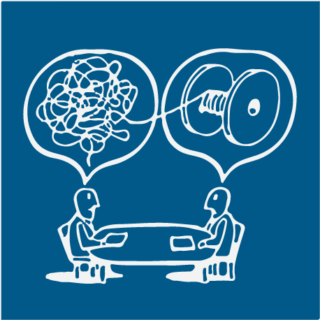
\includegraphics[width=0.7\textwidth]{coaching-square-background-320x320}
	\end{figure}
	\thispagestyle{empty}
	\newpage
	
	\section*{Introduction}
	My coach for the 3rd semester of the Honours program is Cees-Jeroen Bes.\\
	
	During the first coaching session Cees-Jeroen asked me about my current activities within my minor Smart Farming. During this minor, I have to work in different groups every four weeks and our results are based on our group performance.\\
	
	\section{Letting go}
	In our first part of the coaching session we discussed my tendency to take on a lot of work. A part of this behaviour is created by my desire for structure in my work. \\
	
	When a group member creates a report, I often expect it to follow the \textbf{structure} of Grit \cite{Grit2011} and a book called 'De APA-richtlijnen' \cite{Poelmans2013}. \\
	
	I have an increased need for structure relative to my fellow students, because that is part of me and my perfectionism. It is what drives me to excellence. To do my best and try to go beyond. \\
	
	A part of this structure allows me to feel in \textbf{control}. To become a better professional, leader or teamplayer, \underline{trust} in my fellow students is required to be able to let go a part of that control.  \\
	
	Letting go a part of the control makes me expect a certain level of workmanship. Together with Cees-Jeroen I discussed the feeling of disappointment I feel sometimes when a group member does an assignment differently than me. \\
	
	I came to the insight that a part of the disappointment is, that I am giving up a part of the control I have and that this creates a, sometimes unrealistic, expectation towards my fellow student.\\
	
	I, and everybody else, should be proud of the fact that we do not know everything. That there is still room for more knowledge. 
\newpage
\begin{displayquote}
	\textit{"I don't need to know everything I just need to know where to find it when I need it."} \\ Albert Einstein
\end{displayquote}
	
	\section{Agreements}
	Possible solutions to my feelings towards releasing a part of the control, is creating clear agreements. An example of a solution is discussing a deadline with my fellow group member that I can substantiate and where he/she can give their thoughts about my proposal. \\
	
	Together we can make a deadline that we both can agree on and sometimes that means I have to be patient.
		
	\section{Communication}
	A large portion of the agreements consists of communicating with my fellow students in a open and clear way. Nobody should feel like they are held back by each other.\\
	
	Cees-Jeroen explains to me that I should broaden my communication within the research group. Broadening the communication means that I should not only pay extra attention to my communication within my group, but within the whole research group.\\
	
	Cees-Jeroen and I agree that when the communication, that could also be in the form of agreements, is more efficient, the students can focus more on their tasks.\\
	
	There will be less 'wasted' energy in discussing \underline{how} we should communicate and that energy should rather be spend in communication between the students in the form of meetings, reports and/or presentations.
	
	
	\newpage
	\printbibliography
	
\end{document}